\newcommand\thC{\(\theta^1\)\,Ori~C}
\defcitealias{Canto:1996}{CRW}
\newcommand\CRW{\citetalias{Canto:1996}}


\section{Application to the hypersonic thin shell solution}
\label{sec:crw-scenario}
As an example application of the ideas of this paper, we consider a
generalization of the thin-shell solution presented in
\citet[][hereafter \CRW{}]{Canto:1996}, for the interaction of two
hypersonic, constant velocity stellar winds.  It is assumed that the
two shocks are highly radiative and that the post-shock flows are
perfectly mixed to form a single shell of negligible thickness.  In
this approximation, the shape of the shell was found algebraically by
\CRW{} from considering conservation of linear and angular momentum,
following an approach first outlined in \citet{Wilkin:1996a}.  The
shape of the bow shock shell is uniquely determined by the parameter
\(\beta\), defined as the momentum-loss ratio of the two winds:
\begin{equation}
  \label{eq:beta-definition}
  \beta \equiv \frac{\dot{M}_w V_w}{\dot{M}_{w1} V_{w1}} . 
\end{equation}
In this definition we use the terminology of \CRW{}, in which
\(\dot{M}_w\) and \(V_w\) are the mass-loss rate and velocity,
respectively, of the wind with source at the origin, while
\(\dot{M}_{w1}\) and \(V_{w1}\) are the mass-loss rate and velocity of
the second wind, located at a distance \(D\) along their \(z\) axis.
Note that \CRW{}'s \(z\) and \(r\) correspond to \(x\) and \(y\) in
sections~\ref{sec:generic-model} to \ref{sec:conic} of the current
paper.  By always placing the weaker of the two winds at the origin,
it is only necessary to consider \(\beta \le 1\).
 
\begin{figure}
  \centering
  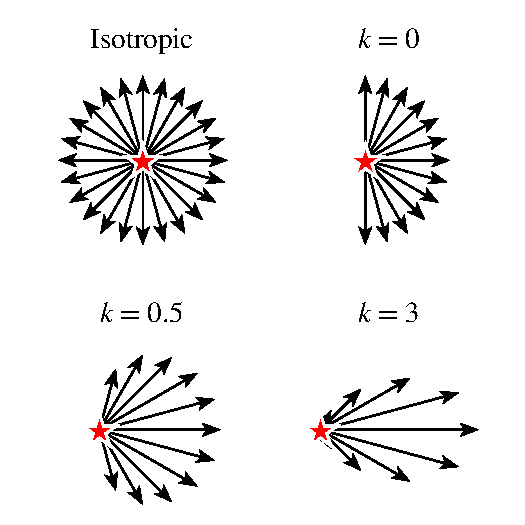
\includegraphics[width=\linewidth]{figs/anisotropic-arrows}
  \caption[]{Schematic diagram of wind flow patterns in isotropic and
    non-isotropic cases.  Arrows represent the wind momentum loss rate
    per solid angle.}
  \label{fig:crw-schema}
\end{figure}
In this work the weakest wind is modeled as an anisotropic hemispherical radial wind
with the following density distribution:
\begin{align}
  n(\theta) = n_0\cos^k\theta
\end{align}  
The index $k$ gives the anisotropy degree. We are interested in winds where $k \geq 0$ for further applications. By the other side, we keep the strongest
wind as isotropic.

The shape of the resultant bow shock is given by:
%If we apply the \CRW{} formalism for a more generalized photoevaporated flow with density given by (\ref{eq:ngen}),
%we find that the solutions for equations (8) - (11) of \CRW{} are the following:

%If we apply the \CRW{} formalism for a generalized photoevaporated flow with density given by equation (\ref{eq:ngen}),
%the shell shape $R(\theta)$ may be calculated from equation (6) of CRW{}:
\begin{align}
  R = \frac{\dot{J}_w + \dot{J}_{w1}}{\left(\dot{\Pi}_{wr}+\dot{\Pi}_{wr1}\right)\cos\theta-\left(\dot{\Pi}_{wz1}+\dot{\Pi}_{wz1}\right)\sin\theta}
  \label{eq:Rmom}
\end{align}

Where:

\begin{align}
\dot{\Pi}_z &= \frac{v_w\dot{M}_w^0}{2(k+2)}\left(1-\cos^{k+2}\theta\right)  \label{eq:pir}\\
\dot{\Pi}_r &= \frac{1}{2}\dot{M}^0_w v_w I_k (\theta) \label{eq:piz}\\
I_k(\theta) & = \int^\theta_0 \cos^k \theta \sin^2\theta~d\theta \label{eq:Ik}\\
\dot{J}_w = 0 \label{eq:jdot} \\
\dot{M}_w &= \frac{\dot{M}_w^0}{2(k+1)}\left(1-\cos^{k+1}\theta\right) \label{eq:dotprop} \\
M^0_w &\equiv 4\pi v_w r^2_{IF} n_0 \bar{m}\\
\dot{\Pi}_{wz1} & = -\frac{\dot{M}^0_{w1}v_{w1}}{4}\sin^2\theta_1\\
\dot{\Pi}_{wr1} & = \frac{\dot{M}^0_{w1}v_{w1}}{4}\left(\theta_1-\sin\theta_1\cos\theta_1\right)\\
\dot{J}_{w1} & = \frac{\dot{M}^0_{w1}v_{w1}}{4}\left(\theta_1-\sin\theta_1\cos\theta_1\right)D \label{eq:jdot1}
\end{align}

Combining equations  (\ref{eq:pir}) to (\ref{eq:jdot1}) we can obtain numerically the bow shock shape $R(\theta)$ from equation (\ref{eq:Rmom}).
To find the projected shape in the plane of sky, we fit $R(\theta)$ into a quadric curve which has the same characteristic radii $(R_0,R_c,R_{90})$. 
%The most notable scenarios, since they have astrophysical relevance are the following:
%$k=1/2$ ak.a. the ``proplyd case'', following \citep{HA:1998}, and $k=0$, ak.a, the ``isotropic case'', following \CRW{}. The comparison between both solutions
%is shown in figure (\ref{fig:r-beta}), along with an extreme anisotropy case. 

\begin{figure}
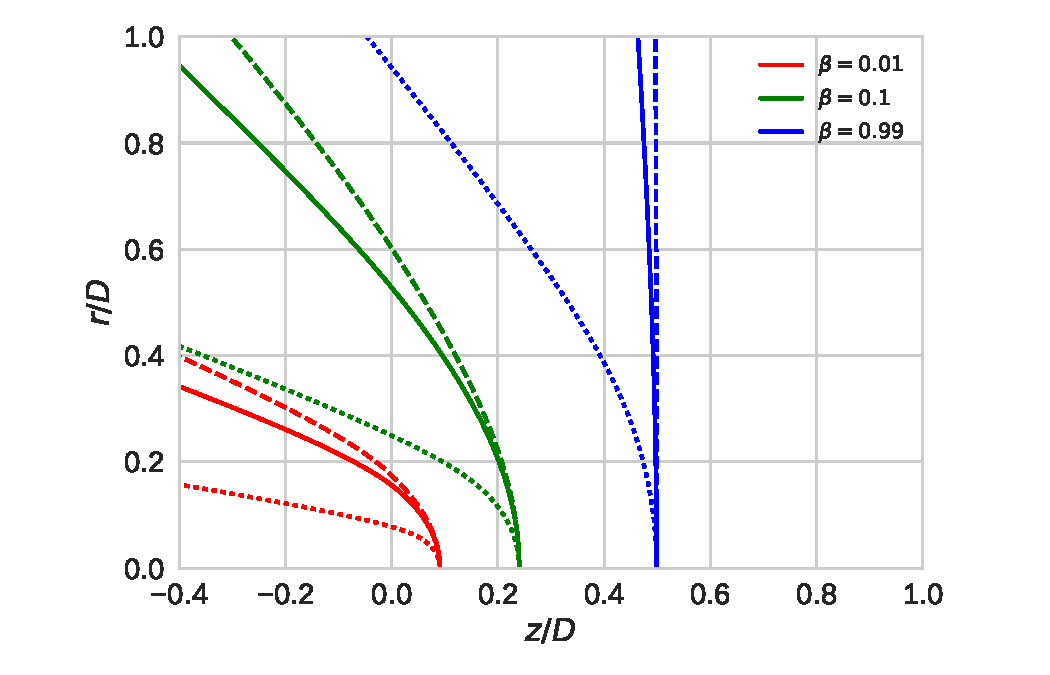
\includegraphics[width=\linewidth]{figs/r-beta}
\caption{Bow shock shapes for interacting winds in the thin-shell
  approximation. Coordinates are normalized by $D$, the distance
  between the two wind sources.  The weaker source is at \((0.0, 0.0)\)
  and the stronger source is at \((1.0, 0.0)\).  Results are shown for
  different values of the wind momentum ratio, \(\beta\), and for the
  case where the weaker wind is isotropic (dashed lines) or an
  anisotropic photoevaporation flow. The solid lines shows a wind with a
  moderate degree of anisotropy $(k=0.5)$, which is expected for the proplyds.
  And the dotted lines show a wind with extreme anisotropy degree $(k=8)$.}
\label{fig:r-beta}
\end{figure}


\subsection{Characteristic Radii}
$R_0$ is obtained directly from equation (27) of \CRW{} as the distance from the inner source where the RAM pressure of the interacting winds is in equilibrium.
%Here goes a little introduction
For the rest of the radii we need a relation between $\theta$ and $\theta_1$ as follows:


\begin{align}
\theta_1\cot\theta_1 -1 = 2\beta I_k(\theta) \cot\theta - \frac{2\beta}{k+2}\left(1-\cos^{k+2}\theta\right)
\label{eq:th1th}
\end{align}

Equation (\ref{eq:th1th}) is reduced to equation (24) of \CRW{} when $k=0$.
We can obtain $R_{90}$ by following the process shown in appendix \ref{app:r90-analytic},
which lead us to a solution for $B \equiv \frac{R_{90}}{R_0}$:

\begin{align}
\tilde{R}_{90} = \frac{\sqrt(3\xi)\left(1+\beta^{1/2}\right)}{(1-\xi\beta)\left(1+\frac{1}{5}\xi\beta\right)^{1/2}}
\label{eq:B}
\end{align}

Now, the solution for $R_c$ is explained in appendix \ref{app:rc-analytic},
which lead us to derive the radius of curvature at the symmetry axis:

\begin{align}
R_c &= R_0\left(1-2\gamma\right)^{-1} \label{eq:Rcurv} \\
\mathrm{where:~} & \gamma = \frac{C_{k\beta}}{1+\beta^{1/2}}+\frac{1}{6}(1-2\beta^{1/2})
\end{align}

Finally, using equations (\ref{eq:Rcurv}) and (\ref{eq:B}) we can estimate the parameter of
conic curves $\theta_c$ as a function of $(\beta,\xi)$ using equation (\ref{eq:Thc})

\begin{align}
\tan^2\theta_c &= \left| \frac{3\xi\left(1+\beta^{1/2}\right)^2}{\left(1-\xi\beta\right)^2\left(1+\frac{1}{5}\xi\beta\right)}-\frac{2}{\left(1-2\gamma\right)}\right| 
\label{eq:thc-CRW}
\end{align}

\begin{figure}
\begin{tabular}{c}
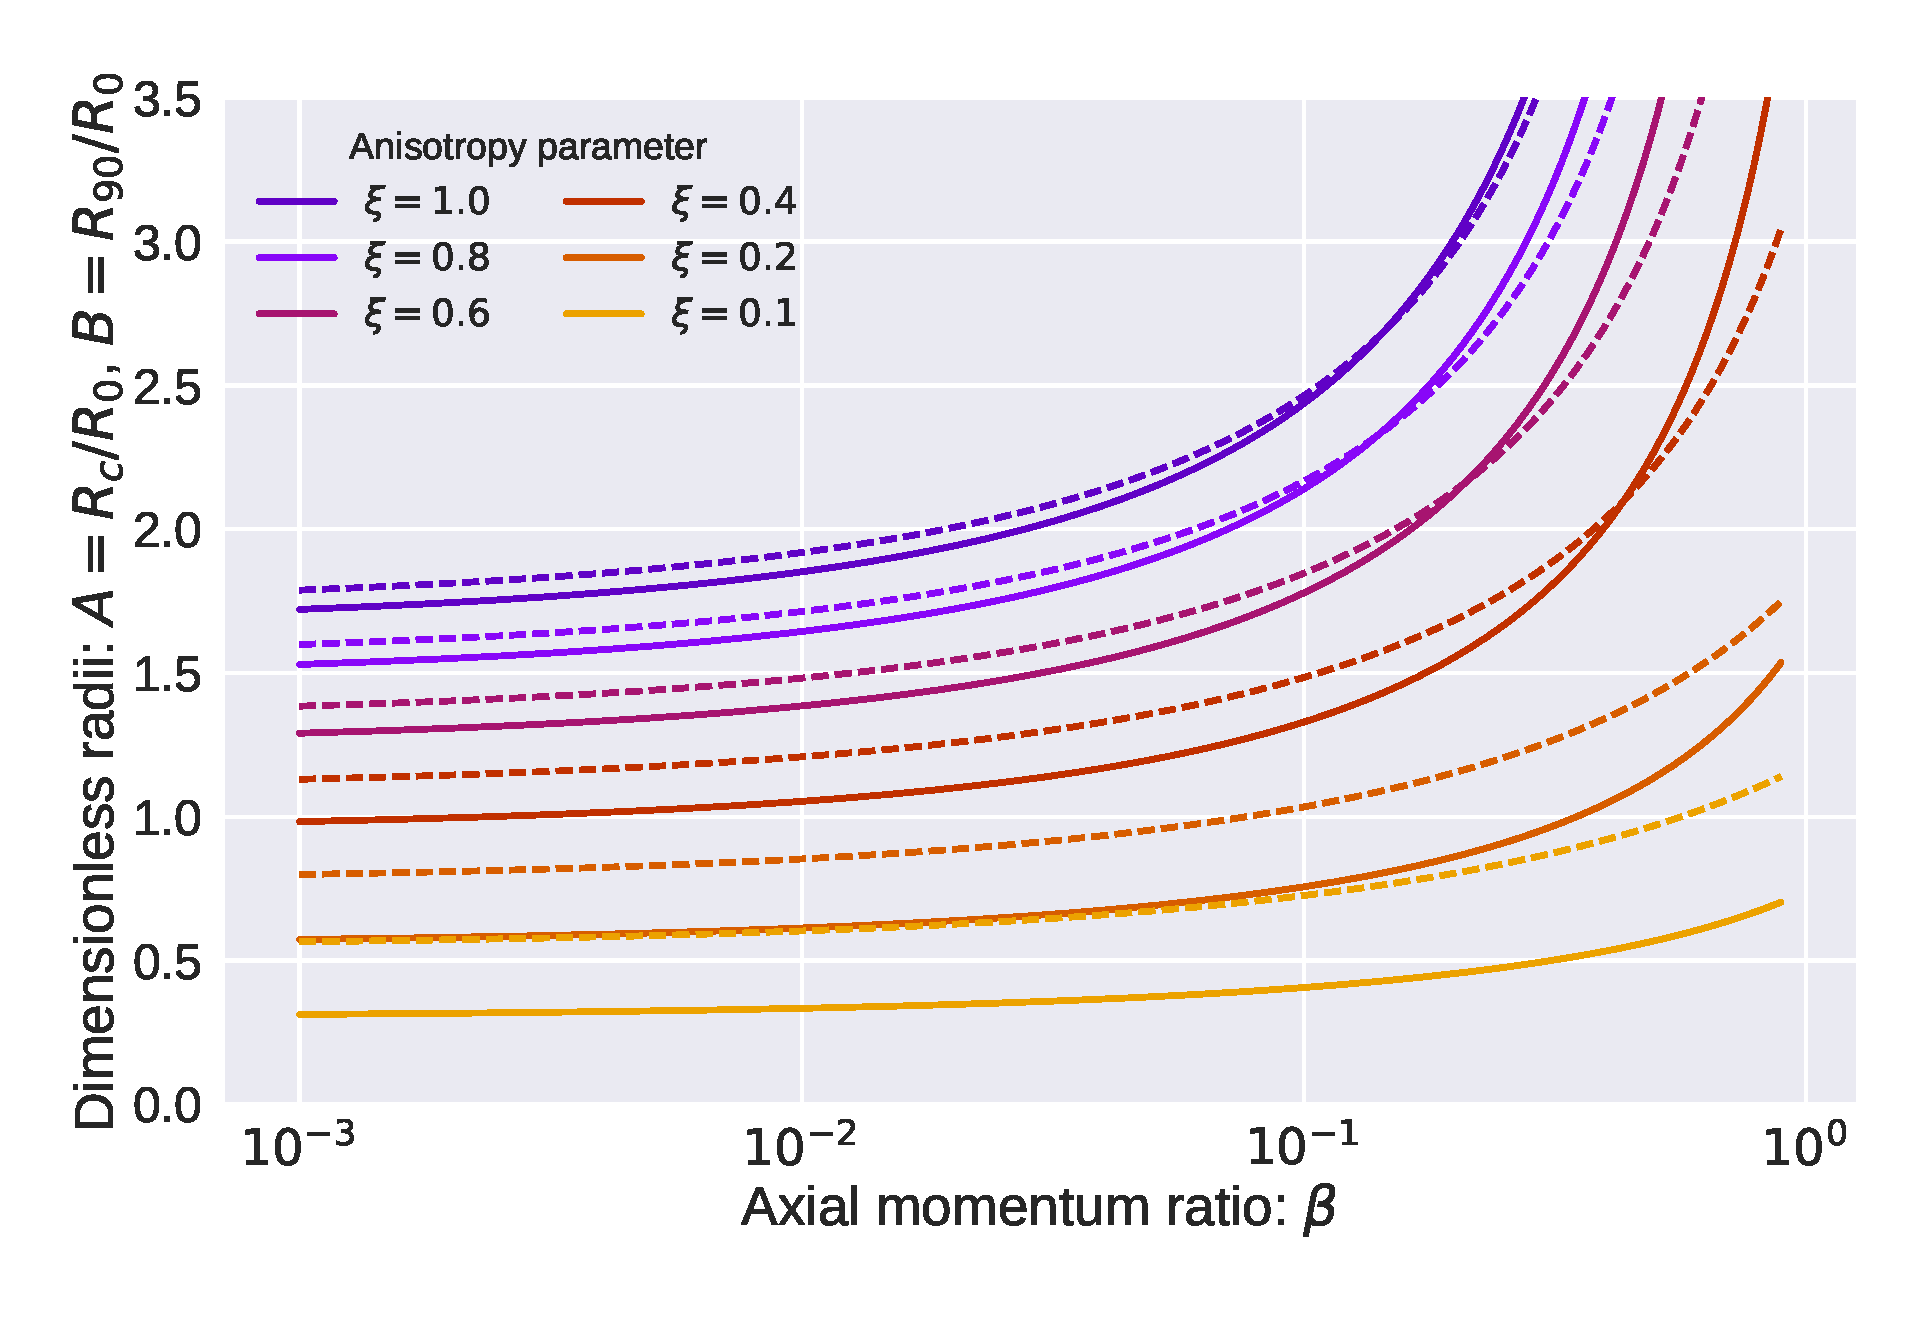
\includegraphics[width=\linewidth]{figs/AB-beta-log} \\
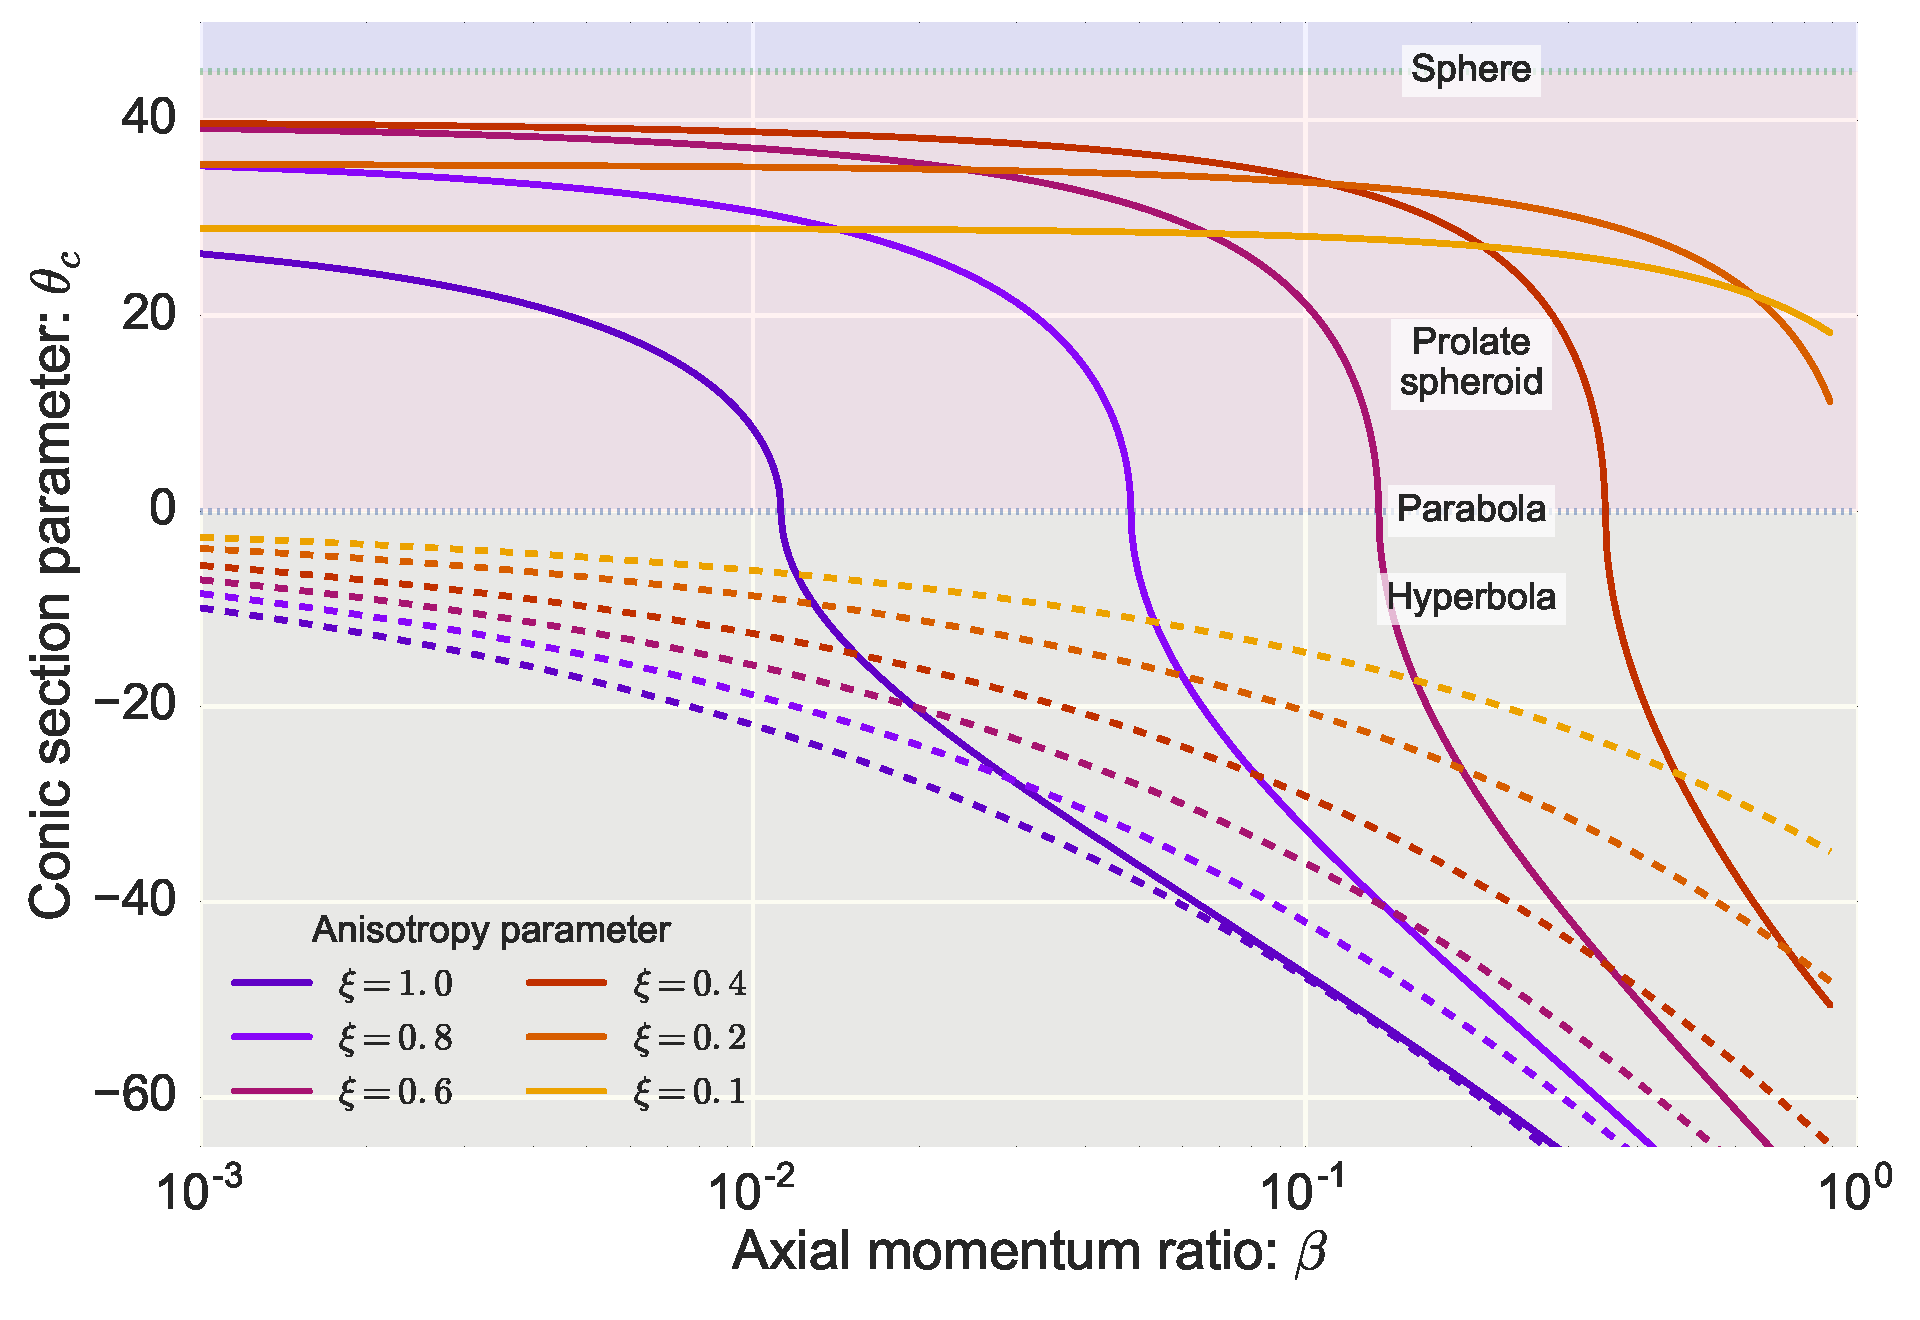
\includegraphics[width=\linewidth]{figs/thc-beta-log}
\end{tabular}
\caption{Top: Characteristic radii, $\tilde{R}_c = R_c/R_0$ (solid lines) and $\tilde{R}_{90}
  = R_{90}/R_0$ (dashed lines)
  vs $\beta$, calculated from quadric fits to the generalized CRW
  solutions with varying degrees of isotropy $\xi$.  Bottom: Conic
  angle $\theta_c$ vs $\beta$ for the bow 
  shock head (solid lines) and the bow shock tail (dashed lines).}
\label{fig:rad-beta}
\end{figure}


% Observationally, we can measure the projected radii. In order to estimate the model parameters is neccesary to measure at least two of the mentioned radii,
%being $R_0$ the
%easiest to measure. Therefore, we may compare both $R_c$ and $R_{90}$ against $R_0$ as shown in figure (\ref{fig:prop-shell-rad}). 

With this we can use the results of section \ref{sec:conic} to estimate the projected conic shapes for bow shocks with different winds 
momenta and different density distributions. Figure \ref{fig:rad-beta} shows equations ( \ref{eq:B}), (\ref{eq:Rcurv}) and (\ref{eq:thc-CRW}) for different anisotropy indexes. 

\subsection{Special Case: Isotropic Wind/Parallel Flow Interaction Problem}

This problem has already been solved in \citet{Wilkin:1996a} and \CRW{}, which have an explicit form for the shell shape, given by:

\begin{align}
  R(\theta) = R_0\csc\theta\left[3(1-\theta\cot\theta)\right]^{1/2} \label{eq:R-Wilkin}
\end{align}
Where:
\begin{align}
  R_0 = \left(\frac{\dot{M}⁰_wv_w}{4\pi\rho_a v_a^2}\right)^{1/2}
\end{align}
And $\rho_a$ and $v_a$ being the density and the velocity of the Parallel wind, respectively.
The characteristic radii are given by:
\begin{align}
  \tilde{R}_{90} &= \sqrt{3} \\
  \tilde{R}_c &= \frac{5}{3}
\end{align}
The derivation of these values is developed in appendix \ref{app:ch-rad-Wilkin}

\subsection{Fits to the tail}
\label{sec:fits-tail}

In most cases, the quadric fit to the head of the bowshock does a very poor job of representing the ``wings'' or ``tail''.  The bowshock tail in all cases is asymptotically hyperbolic, with 

We therefore 
We carry out three-level nested fits to determine the 

For the hyperbola ``center''
\begin{multline}
  \label{eq:tail-analytic-x0}
  x_{0,\mathrm{t}} = 0.7 \beta^{-0.55} \biggl[
    C_3 \bigl(\log_{10}\beta\bigr)^3 + C_2 \bigl(\log_{10}\beta\bigr)^2 
  \\ + C_1 \log_{10}\beta + C_0
  \biggr]
\end{multline}
\begin{equation}
  \label{eq:tail-analytic-x0-minus-a}
  (x_{0,\mathrm{t}} - a_{\mathrm{t}}) = D_2 (\log_{10}\beta)^2 + D_1 \log_{10}\beta + D_0
\end{equation}
where
\begin{alignat}{2}
  \label{eq:tail-analytic-coeffs-c}
  C_k &= c_{2,k} \xi^2 + c_{1,k} \xi + c_{0,k} &\quad \text{for\ } k &= \{0, 1, 2, 3\} \\
  \label{eq:tail-analytic-coeffs-d}
  D_k &= d_{2,k} \xi^2 + d_{1,k} \xi + d_{0,k} &\quad \text{for\ } k &= \{0, 1, 2\}
\end{alignat}


\newcommand\iso{\ensuremath{^{\mathrm{iso}}}}

\begin{table}
  \caption{Coefficients for hyperbola fit to bowshock tails}
  \label{tab:tail-fit-coeffs}
  \renewcommand\arraystretch{1.2}
  \setlength\tabcolsep{0.5\tabcolsep}
  \begin{tabular}{@{}llll@{}}
    \toprule
    Equation~(\ref{eq:tail-analytic-x0}) & 
    \multicolumn{3}{l}{
    Equation~(\ref{eq:tail-analytic-coeffs-c}) \dotfill
    } \\ \midrule
    \( C\iso_0 = +1.3195     \)    
    & \( c_{0,0} = +2.0758   \)  
    & \( c_{1,0} = -0.2309   \)  
    & \( c_{2,0} = -0.2532   \)\\
      \( C\iso_1 = +0.4229     \)    
    & \( c_{0,1} = +0.9571   \)  
    & \( c_{1,1} = -0.1530   \)  
    & \( c_{2,1} = -0.2487   \)\\
      \( C\iso_2 = +0.1092     \)    
    & \( c_{0,2} = +0.2528   \)  
    & \( c_{1,2} = -0.0360   \)  
    & \( c_{2,2} = -0.0794   \)\\
      \( C\iso_3 = +0.0051     \)    
    & \( c_{0,3} = +0.0171   \)  
    & \( c_{1,3} = -0.0010   \)  
    & \( c_{2,3} = -0.0095   \)\\ \midrule
    Equation~(\ref{eq:tail-analytic-x0-minus-a}) &
    \multicolumn{3}{l}{
    Equation~(\ref{eq:tail-analytic-coeffs-d}) \dotfill
    } \\ \midrule
    \( D\iso_0 = +0.7962   \)    
    & \( d_{0,0} = +0.8516 \)  
    & \( d_{1,0} = -0.0907 \)  
    & \( d_{2,0} = -0.2002 \)\\
      \( D\iso_1 = -0.2363   \)    
    & \( d_{0,1} = -0.7620 \)  
    & \( d_{1,1} = +0.1411 \)  
    & \( d_{2,1} = -0.0295 \)\\
      \( D\iso_2 = -0.0126   \)    
    & \( d_{0,2} = -0.0683 \)  
    & \( d_{1,2} = +0.0390 \)  
    & \( d_{2,2} = -0.0236 \)\\
    \bottomrule
  \end{tabular}
\end{table}




\begin{figure*}
  \centering
  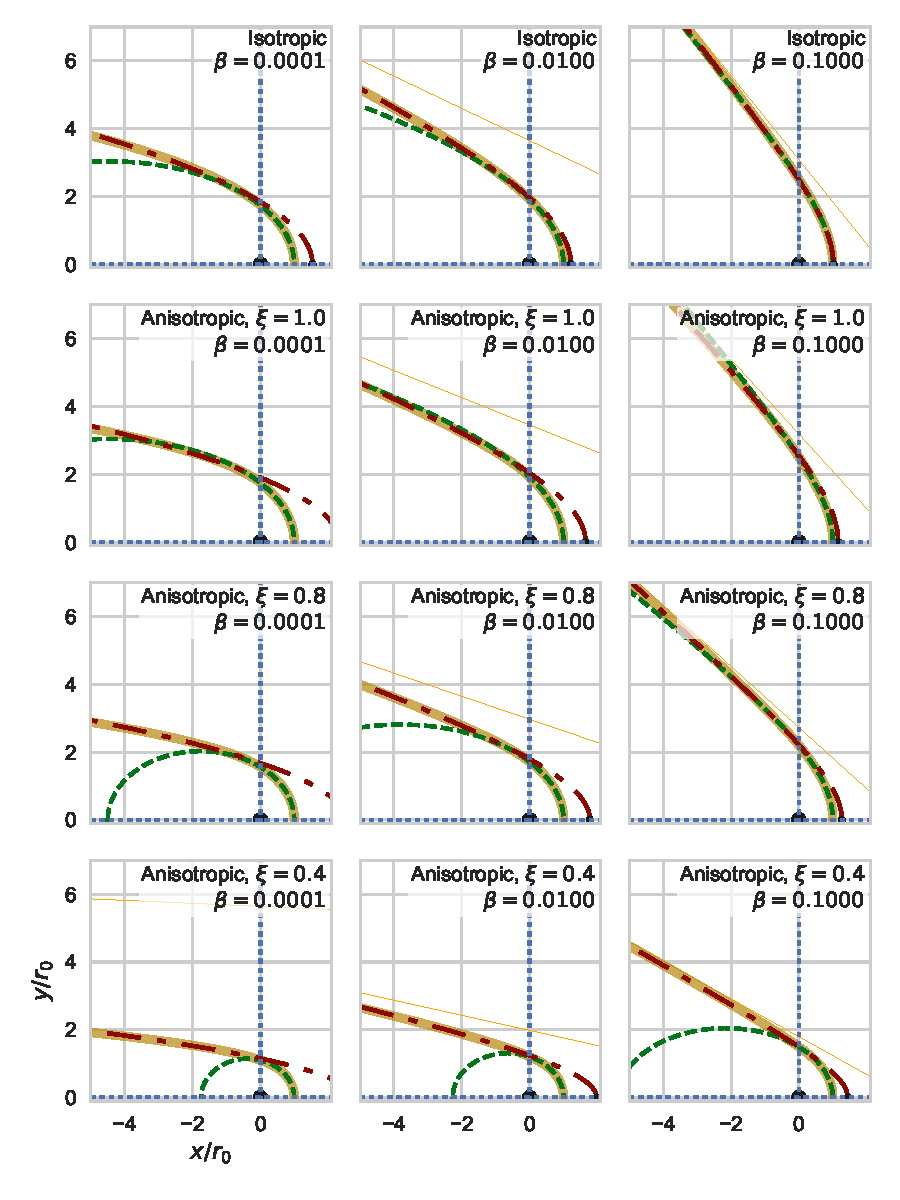
\includegraphics[width=0.8\textwidth]{figs/conic-head-tail-analytic}
  \caption{Double quadric fits to thin shell
    solutions.}
  \label{fig:head-tail}
\end{figure*}

\begin{figure*}
  \centering
  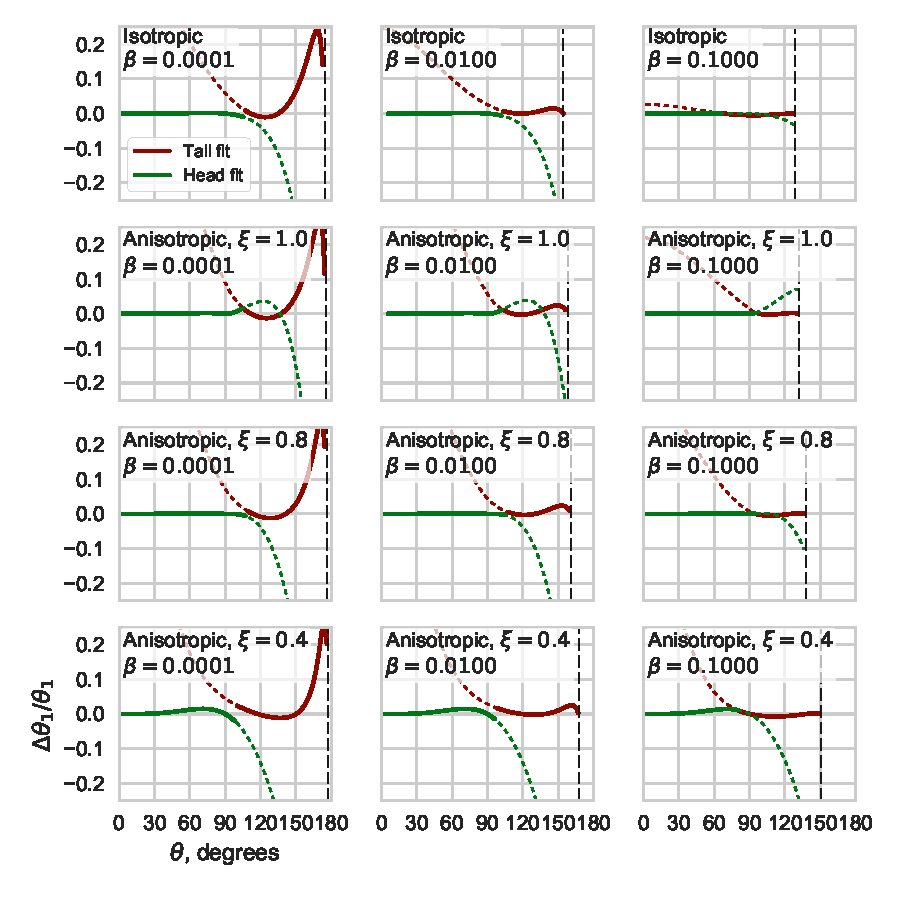
\includegraphics[width=0.8\textwidth]{figs/conic-head-tail-residuals}
  \caption[]{Residuals of double quadric fits to thin shell solutions.
    Residuals are expressed as the fractional error in the
    complementary angle \(\theta_1\) for the same parameters as are shown
    in Fig.~\ref{fig:head-tail}.}
  \label{fig:head-tail-residuals}
\end{figure*}

\subsection{Projection effects in the thin shell model}
\label{sec:proj-effects-thin}

\begin{figure}
  \centering
  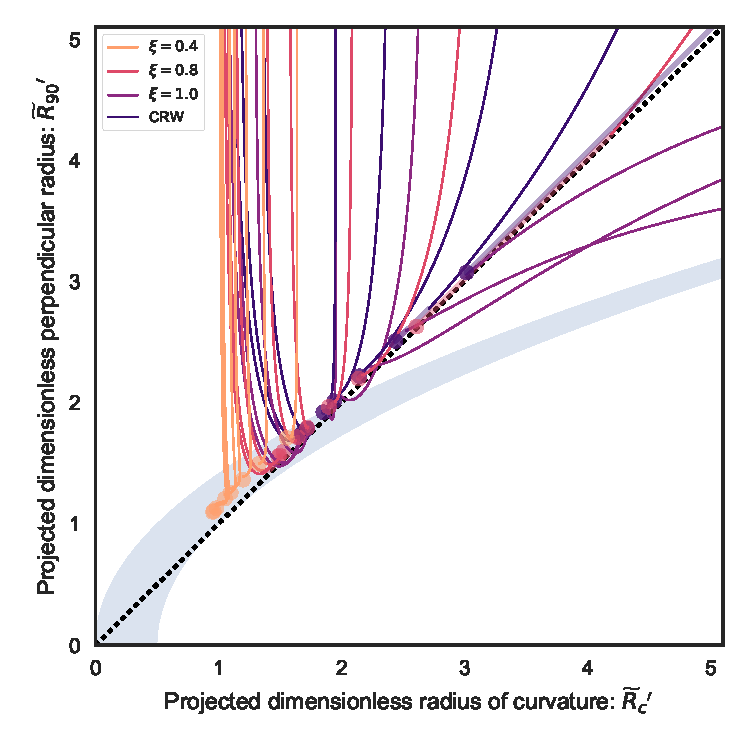
\includegraphics[width=\linewidth]{figs/two-quadric-R90-vs-Rc}
  \caption{Diagnostic diagram for thin shell models}
  \label{fig:thin-shell-R90-Rc}
\end{figure}

\begin{figure*}
  \centering
  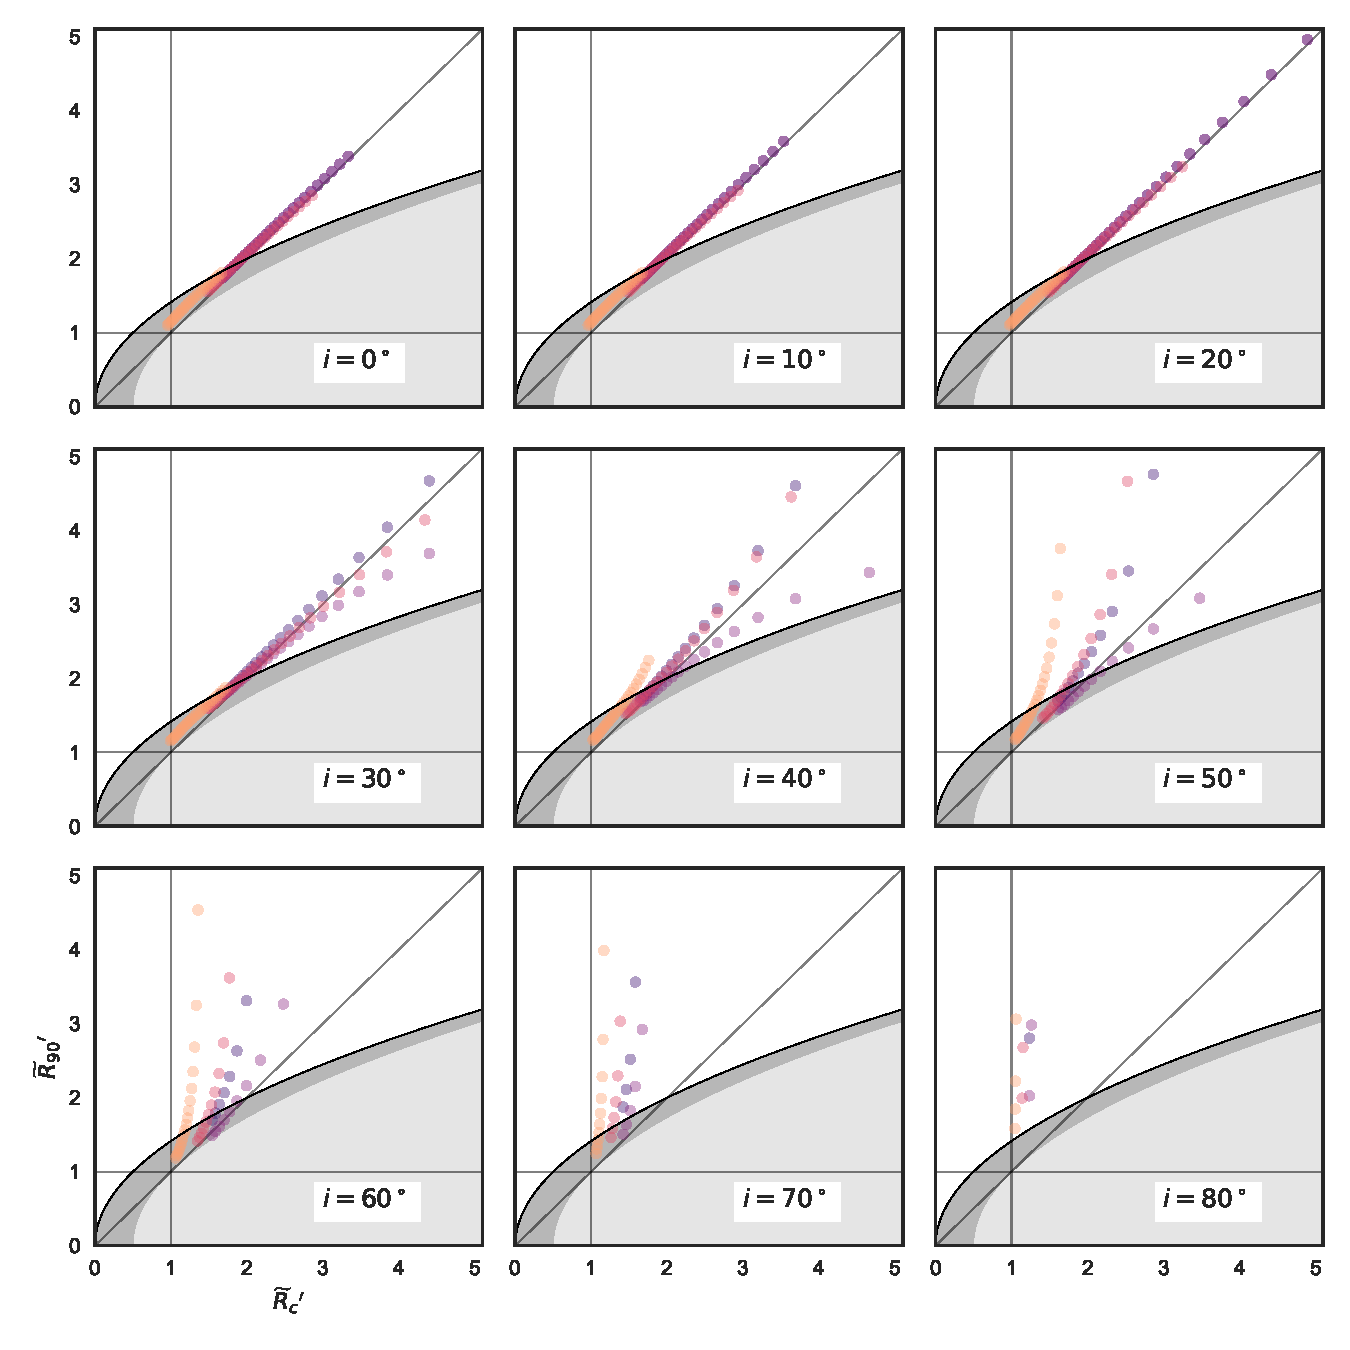
\includegraphics[width=0.8\textwidth]{figs/two-quadric-R90-Rc-snapshots}
  \caption{Variation with inclination angle of radii diagnostics}
  \label{fig:thin-shell-R90-Rc-snapshots}
\end{figure*}


%%% Local Variables:
%%% mode: latex
%%% TeX-master: "quadrics-bowshock"
%%% End:
